\section{Referencia de la Clase Articulo\-View}
\label{classArticuloView}\index{ArticuloView@{ArticuloView}}
Muestra la ventana de art\'{\i}culos.  


{\tt \#include $<$articuloview.h$>$}

Diagrama de herencias de Articulo\-View\begin{figure}[H]
\begin{center}
\leavevmode
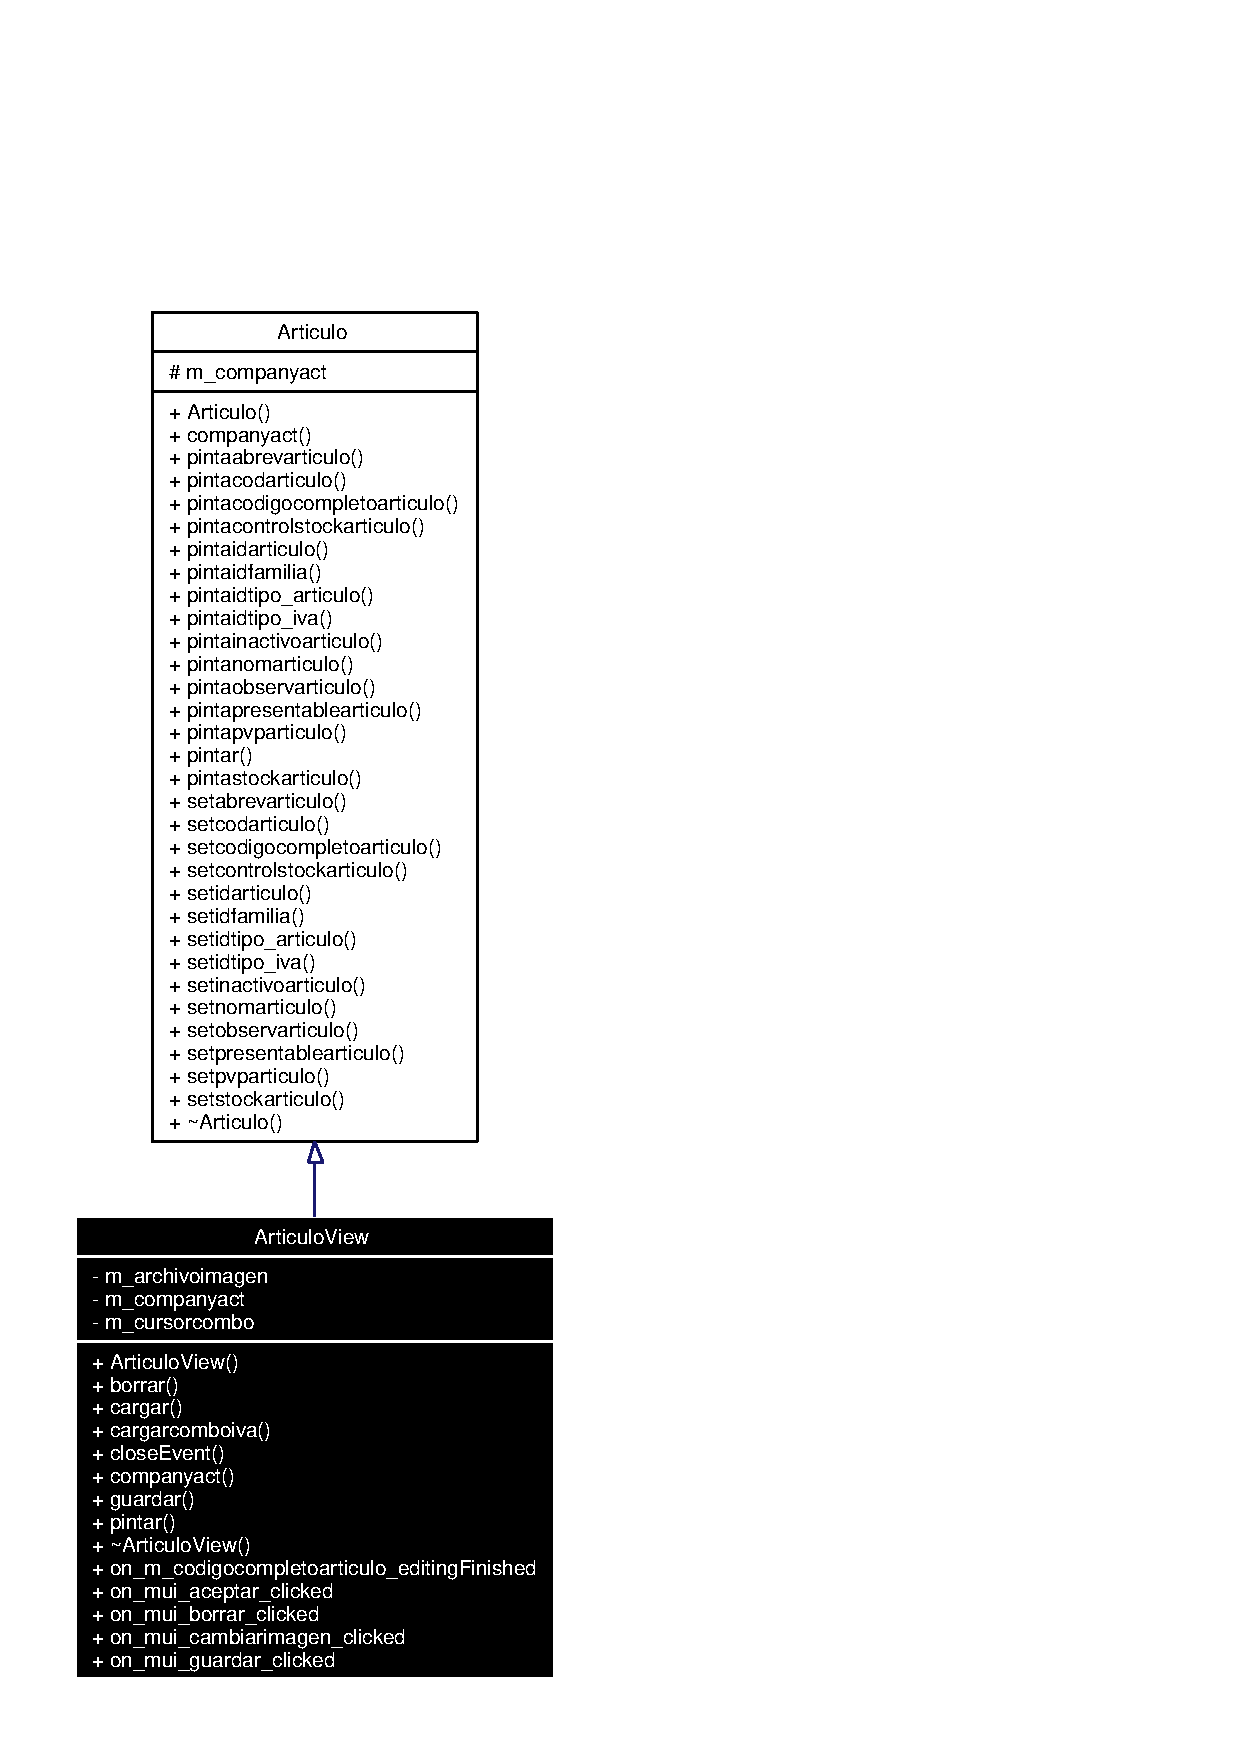
\includegraphics[width=133pt]{classArticuloView__inherit__graph}
\end{center}
\end{figure}
Diagrama de colaboraci\'{o}n para Articulo\-View:\begin{figure}[H]
\begin{center}
\leavevmode
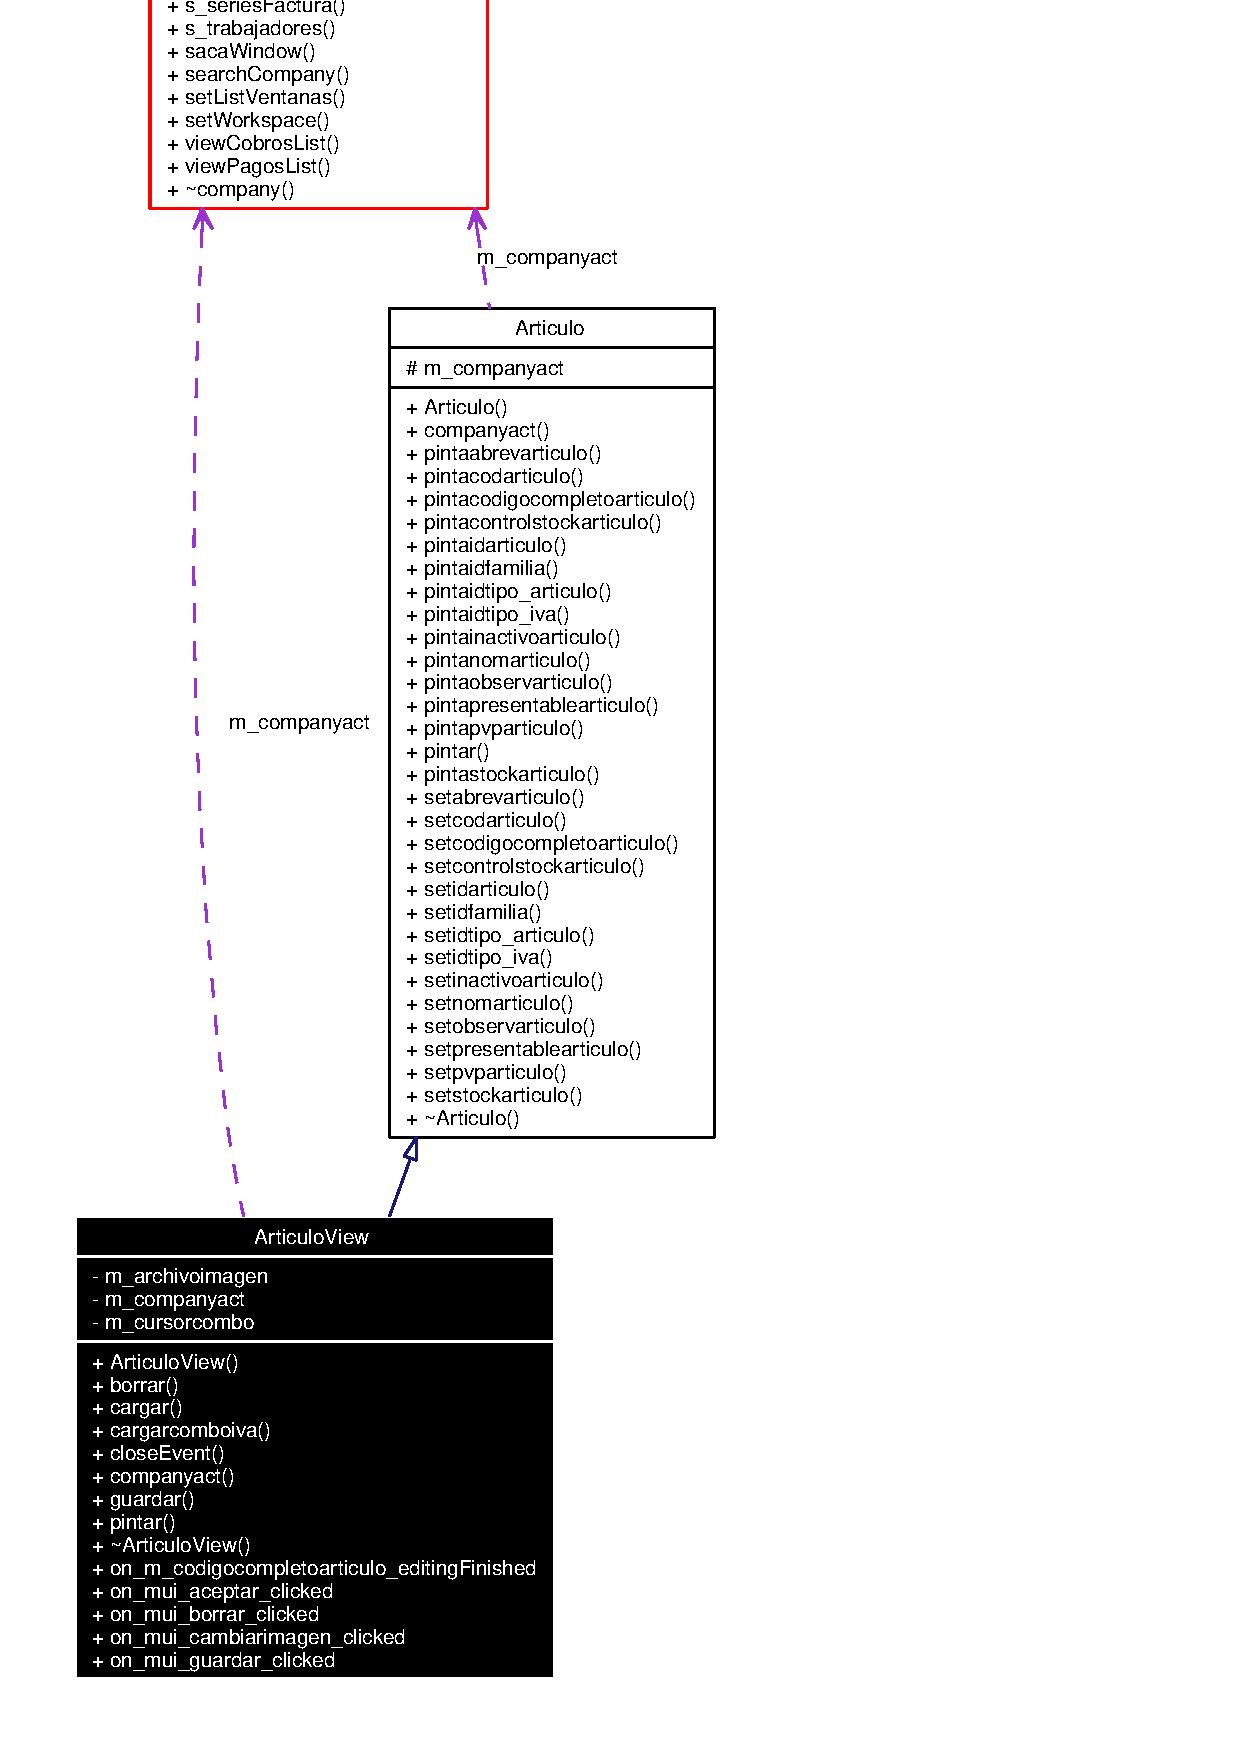
\includegraphics[width=172pt]{classArticuloView__coll__graph}
\end{center}
\end{figure}
\subsection*{Slots p\'{u}blicos}
\begin{CompactItemize}
\item 
virtual void {\bf on\_\-m\_\-codigocompletoarticulo\_\-editing\-Finished} ()\label{classArticuloView_i0}

\item 
virtual void {\bf on\_\-mui\_\-aceptar\_\-clicked} ()\label{classArticuloView_i1}

\item 
virtual void {\bf on\_\-mui\_\-borrar\_\-clicked} ()\label{classArticuloView_i2}

\begin{CompactList}\small\item\em Esta funcion se ejecuta cuando se ha pulsado sobre el boton de borrar. \item\end{CompactList}\item 
virtual void {\bf on\_\-mui\_\-cambiarimagen\_\-clicked} ()\label{classArticuloView_i3}

\item 
virtual void {\bf on\_\-mui\_\-guardar\_\-clicked} ()\label{classArticuloView_i4}

\end{CompactItemize}
\subsection*{M\'{e}todos p\'{u}blicos}
\begin{CompactItemize}
\item 
{\bf Articulo\-View} ({\bf company} $\ast$emp, QWidget $\ast$parent=0)
\item 
int {\bf borrar} ()
\item 
int {\bf cargar} (QString)
\item 
int {\bf cargarcomboiva} (QString)\label{classArticuloView_a3}

\begin{CompactList}\small\item\em Hace la carga del combo-box de tipos de iva para el articulo. \item\end{CompactList}\item 
void {\bf close\-Event} (QClose\-Event $\ast$)\label{classArticuloView_a4}

\item 
{\bf company} $\ast$ {\bf companyact} ()\label{classArticuloView_a5}

\item 
int {\bf guardar} ()
\item 
void {\bf pintar} ()
\end{CompactItemize}


\subsection{Descripci\'{o}n detallada}
Muestra la ventana de art\'{\i}culos. 



\subsection{Documentaci\'{o}n del constructor y destructor}
\index{ArticuloView@{Articulo\-View}!ArticuloView@{ArticuloView}}
\index{ArticuloView@{ArticuloView}!ArticuloView@{Articulo\-View}}
\subsubsection{\setlength{\rightskip}{0pt plus 5cm}Articulo\-View::Articulo\-View ({\bf company} $\ast$ {\em comp}, QWidget $\ast$ {\em parent} = {\tt 0})}\label{classArticuloView_a0}


Disparamos los plugins. 

\subsection{Documentaci\'{o}n de las funciones miembro}
\index{ArticuloView@{Articulo\-View}!borrar@{borrar}}
\index{borrar@{borrar}!ArticuloView@{Articulo\-View}}
\subsubsection{\setlength{\rightskip}{0pt plus 5cm}int Articulo\-View::borrar ()}\label{classArticuloView_a1}


Disparamos los plugins \index{ArticuloView@{Articulo\-View}!cargar@{cargar}}
\index{cargar@{cargar}!ArticuloView@{Articulo\-View}}
\subsubsection{\setlength{\rightskip}{0pt plus 5cm}int Articulo\-View::cargar (QString {\em idarticulo})}\label{classArticuloView_a2}


Esta funcion carga un articulo de la base de datos y lo presenta. Si el parametro pasado no es un identificador valido entonces se pone la ventana de edicion en modo de insercion.

Disparamos los plugins.

Cambiamos el titulo de la ventana para que aparezca el codigo del articulo. \index{ArticuloView@{Articulo\-View}!guardar@{guardar}}
\index{guardar@{guardar}!ArticuloView@{Articulo\-View}}
\subsubsection{\setlength{\rightskip}{0pt plus 5cm}int Articulo\-View::guardar ()}\label{classArticuloView_a6}


Metodo de guardar la ficha. Guarda todos los componentes de la ficha. Si todo ha ido bien devuelve 0 Si hay algun error debe ser tratado con el manejo de excepciones catch.

Guardamos la imagen, si es que existe.

Guardamos la lista de componentes.

Disparamos los plugins \index{ArticuloView@{Articulo\-View}!pintar@{pintar}}
\index{pintar@{pintar}!ArticuloView@{Articulo\-View}}
\subsubsection{\setlength{\rightskip}{0pt plus 5cm}void Articulo\-View::pintar ()\hspace{0.3cm}{\tt  [virtual]}}\label{classArticuloView_a7}


Pintamos el stockable y el presentable. 

Reimplementado de {\bf Articulo} {\rm (p.\,\pageref{classArticulo_a15})}.

La documentaci\'{o}n para esta clase fu\'{e} generada a partir de los siguientes archivos:\begin{CompactItemize}
\item 
articuloview.h\item 
articuloview.cpp\end{CompactItemize}
